\documentclass{beamer}

\usecolortheme[dark,accent=cyan]{solarized}

\beamertemplatenavigationsymbolsempty

\usepackage{graphicx}
\usepackage{hyperref}
\usepackage{colortbl, xcolor}
\usepackage{booktabs}

\usepackage{tikz}
\usetikzlibrary{calc}

\usepackage{minted}
\usemintedstyle{native}
\definecolor{DarkGray}{gray}{0.1}
\definecolor{DarkGray}{gray}{0.1}

\usepackage{amsmath} % a package for building a matrix
\usetikzlibrary{plotmarks} % a package for building line plots using defined data sets
\usepackage{pgfplots}

\usetikzlibrary{positioning,calc}
\usetikzlibrary{automata}
\usepackage{pstricks}

\title{Defection and Cooperation amongst Prisoners}
\author{@NikoletaGlyn}
\date{}
\institute[]
{
\begin{center}
    
\includegraphics[width=.15\textwidth]{static/cardiff_uni_logo.jpg}
\end{center}
}

\begin{document}

\frame{\titlepage}

\begin{frame}{}
    \begin{center}
        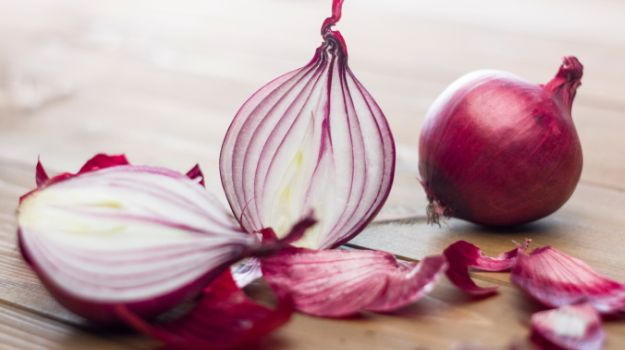
\includegraphics[width=.80\textwidth]{static/onion.jpg}
    \end{center}
\end{frame}

\begin{frame}{}
    \begin{figure}[htp]
        \centering
                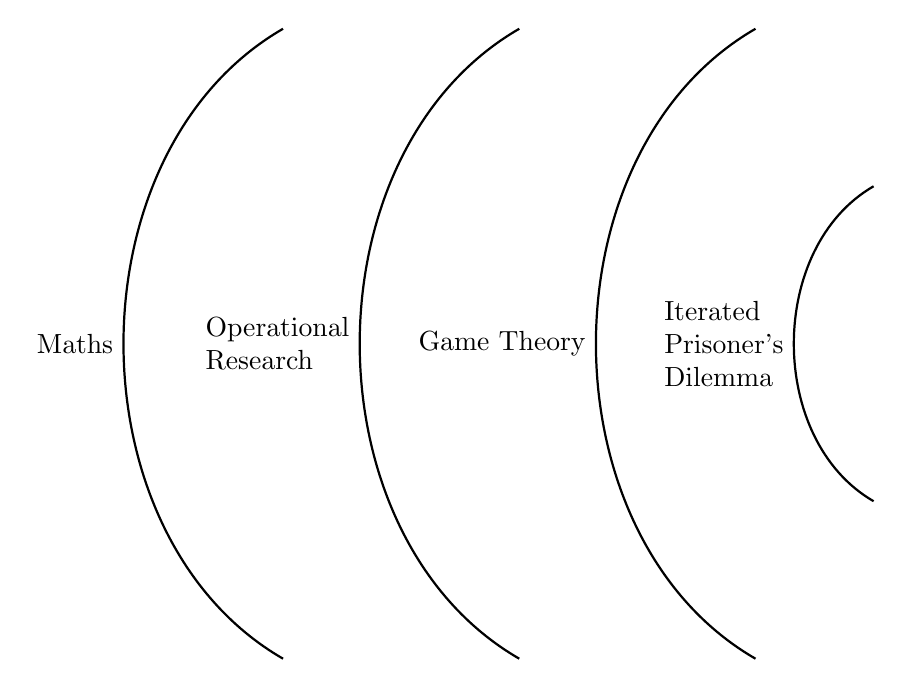
\begin{tikzpicture}
                    \draw [thick] (-2,2) to [bend left=60] node[midway, left] {Maths} (-2,10);
                    \draw [thick] (1,2) to [bend left=60] node[midway, align=left, left] {Operational\\Research}(1,10);
                    \draw [thick] (4,2) to [bend left=60] node[midway, left] {Game Theory} (4,10);
                    \draw [thick] (5.5,4) to [bend left=60] node[midway, left, align=left] {Iterated\\Prisoner's\\Dilemma} (5.5,8);
                \end{tikzpicture}
    \end{figure}
\end{frame}

\begin{frame}
\begin{center}
\Huge{Operational Research}
\end{center}
\end{frame}

\begin{frame}
    \begin{center}
    \tikzstyle{arrow} = [->,>=stealth]

\begin{tikzpicture}
     \node[align=center, minimum size=2cm] (center) at (0,0) {Operational \\ Research};

    \node[align=center, minimum size=2cm] (v_1) at (360/6 * 1:4cm) {\color{yellow!79}Computing};
    \node[align=center, minimum size=2cm] (v_2) at (360/6 * 2:4cm) {\color{yellow!79}Marketing};
    \node[align=center, minimum size=2cm] (v_6) at (360/6 * 6:4cm) {\color{yellow!79}Optimization};
    \node[align=center, minimum size=2cm] (v_3) at (360/6 * 3:4cm) {\color{yellow!79}Simulation};
    \node[align=center, minimum size=2cm] (v_4) at (360/6 * 4:4cm) {\color{yellow!79} ...};
    \node[align=center, minimum size=2cm] (v_5) at (360/6 * 5:4cm) {\color{yellow!79} ...};

\foreach \phi in {1,...,6}{
     \draw[arrow] [yellow!70] (v_\phi) -- (center);
     \draw[arrow] [yellow!70] (center) -- (v_\phi);
     }
\end{tikzpicture}
    \end{center}
\end{frame}

\begin{frame}
\begin{center}
\Huge{Game Theory}
\end{center}
\end{frame}

\begin{frame}
\begin{center}
\Huge{Traveller's Dilemma}
\end{center}
\end{frame}

\begin{frame}{}
 \Huge
 \[
\begin{bmatrix}
  (2,2) & (4,0) & (4,0)  \\
  (0,4) & (3,3) & (5,1) \\
  (0,4) & (1,5) & (4,4)
\end{bmatrix}
\]
\end{frame}

\begin{frame}
    \begin{center}
        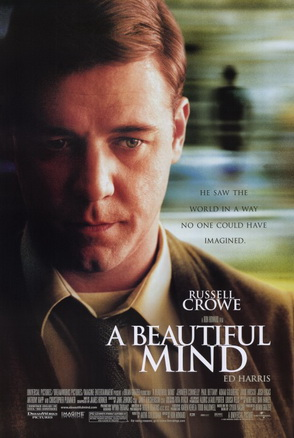
\includegraphics[width=0.4\textwidth]{static/russel.jpg}
    \end{center}
\end{frame}

\begin{frame}
    \begin{center}
        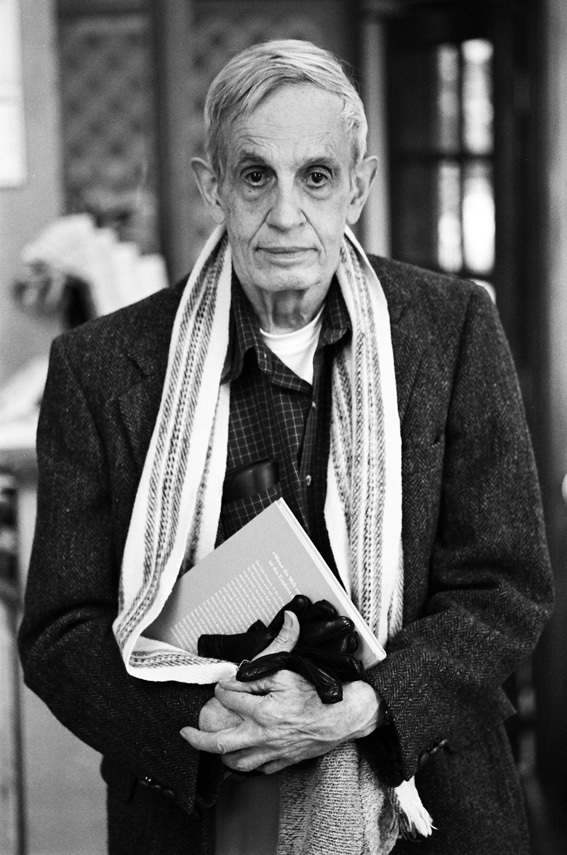
\includegraphics[width=0.4\textwidth]{static/john_nash.jpg}
    \end{center}
\end{frame}


\begin{frame}{}
 \Huge
 \[
\begin{bmatrix}
  (2,2) & (4,0) & (4,0)  \\
  (0,4) & (3,3) & (5,1) \\
  (0,4) & (1,5) & (4,4)
\end{bmatrix}
\]
\end{frame}

\begin{frame}
\begin{center}
\Huge{The Prisoner's Dilemma}
\end{center}
\end{frame}

\begin{frame}
    \begin{center}
        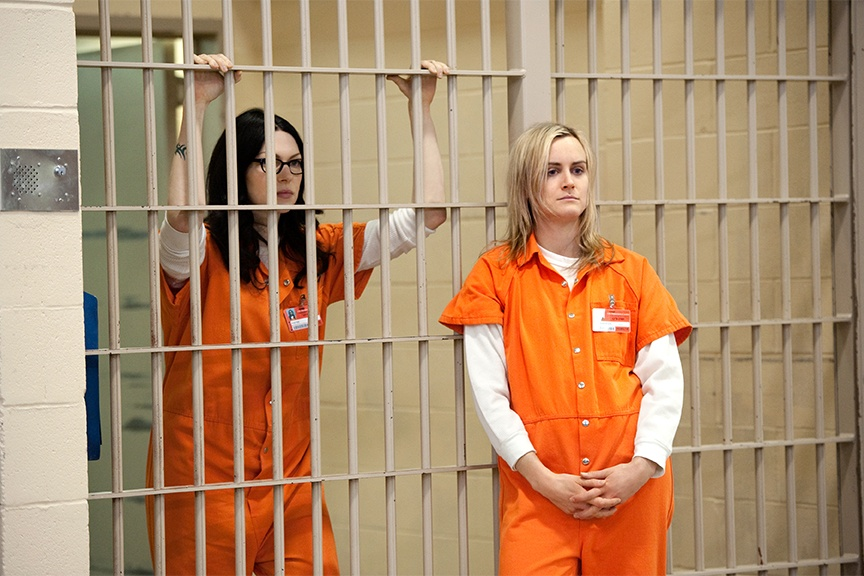
\includegraphics[width=1\textwidth]{static/prisoners.jpg}
    \end{center}
\end{frame}

\begin{frame}{}
 \Huge
 \[
\begin{bmatrix}
  (3,3) & (0,5)  \\
  (5,0) & (1,1)
\end{bmatrix}
\]
\end{frame}

\begin{frame}
    \begin{center}
      \Large{ Robert Axelrod} \\
      \Large{ 1980a: 14+1 strategies} \\
      \Large{ 1980b: 64+1 strategies}

    \end{center}
\end{frame}

\begin{frame}[fragile]{}
	\begin{center}
		\begin{minipage}{0.8\textwidth}
			\begin{minted}
[
frame=lines,
framesep=2mm,
baselinestretch=1.2,
fontsize=\tiny,
bgcolor=DarkGray,
]
{python}

class TitForTat(Player):
    """
    A player starts by cooperating and then mimics the previous action of
    the opponent.

    Note that the code for this strategy is written in a fairly verbose
    way. This is done so that it can serve as an example strategy for
    those who might be new to Python.

    Names:

    - Rapoport's strategy: [Axelrod1980]_
    - TitForTat: [Axelrod1980]_
    """

    def strategy(self, opponent):
        """This is the actual strategy"""
        # First move
        if not self.history:
            return C
        # React to the opponent's last move
        if opponent.history[-1] == D:
            return D
        return C
			\end{minted}
		\end{minipage}
	\end{center}
\end{frame}

\begin{frame}{}
\def\labellist{{" ","(1980)","(1991)","(1992)","(2012)"," ","(2015)"," "}}
    \begin{tikzpicture}
            \begin{axis}[
                height=8cm,
                width=12cm,
                axis lines=left,
                xtick=\empty,
                ytick=\empty,
                nodes near coords={
                                    \pgfmathparse{\labellist[\coordindex]}%
                                    \pgfmathresult }
                ]
    \addplot[color=white,mark=x]
        coordinates{
            (1,1)
            (2,1.1)
            (3,6)
            (4,6.5)
            (5,8.5)
            (6,9)
            (7,9.5)
            (8,12) };
            \end{axis}
    \end{tikzpicture}
\end{frame}

\begin{frame}
    \begin{center}
        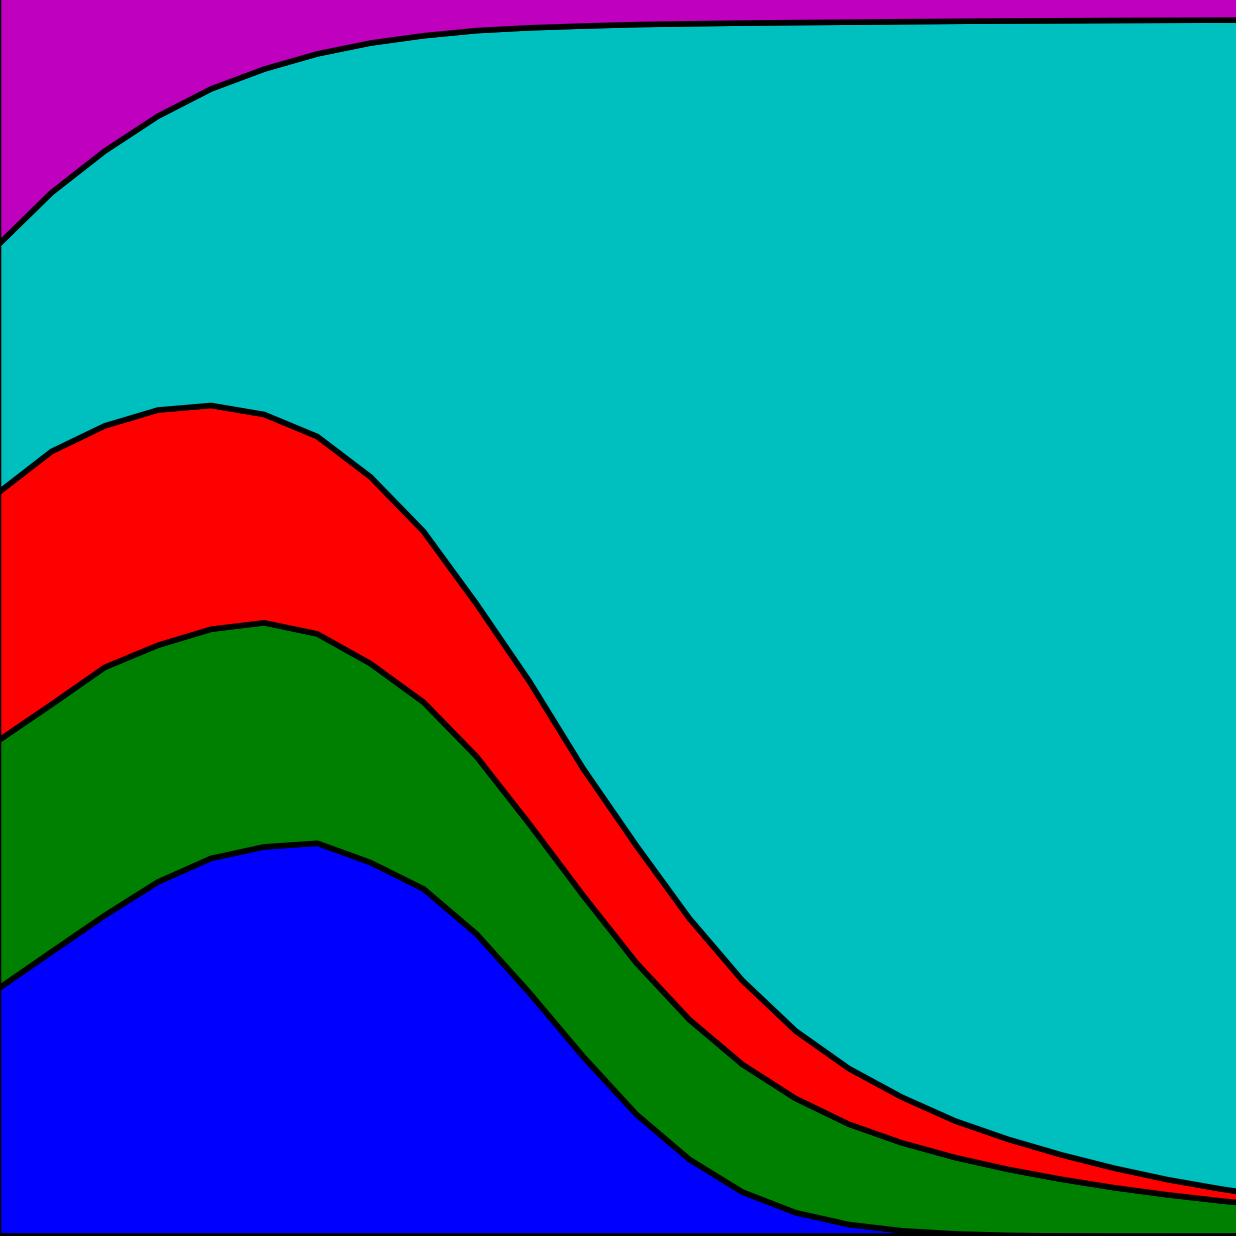
\includegraphics[width=0.4\textwidth]{static/axelrod-logo.png}
    \end{center}
\end{frame}

\begin{frame}
\begin{center}
    \Large{Literature Review} \\
    \Large{Meta study of tournaments} \\
    \Large{Machine learning strategies} \\
    \Large{Evolution}
\end{center}
\end{frame}
\begin{frame}
	\begin{center}
		\small{@NikoletaGlyn}\\
		\small{https://github.com/Nikoleta-v3}\\
		\small{https://github.com/Axelrod-Python/Axelrod}
	\end{center}
\end{frame}

\end{document}

